\documentclass[12pt,titlepage]{article}
\usepackage{fullpage}
\usepackage{epsfig}
\begin{document}
\title{DepGraphAPI Programmer's Guide \\ Release 0.9b}
\author{Paradyn Parallel Performance Tools}
\maketitle
\tableofcontents
\section{Introduction}

The DepGraphAPI is a multi-platform library for creating and analyzing
dependence graph representations of binary code. These graph
representations include data dependence graph (DDG), control
dependence graph (CDG), program dependence graph (PDG), and extended program
dependence graph (xPDG). A data dependence graph provides information about
use-define chains in a function. A control dependence graph is composed of
edges where the execution of the source determines whether the target of this
edge will be executed. A program dependence graph is simply the
combination of this two graphs. Finally, an extended program dependence graph
is an extension to the PDG with extra dependencies used for creating executable
slices.

The current beta of the DepGraphAPI depends on the InstructionAPI library
and the DyninstAPI; future versions will depend only on the
InstructionAPI and ParsingAPI libraries released as part of the
DyninstAPI. Currently we support the IA-32 and AMD-64 architectures as
these are the only architectures supported by the
InstructionAPI. Future architecture support includes PPC, IA-64, and
SPARC; the DepGraphAPI has no file format or operating system
constraints.

The main goal of this API is to provide the user with abstractions
representing the logical dependencies between instructions in a
program. An abstract interface provides two benefits: it simplifies
the development of a tool since the complexity of a particular
architecture is hidden, and it allows tools to easily be ported
between platforms. We use graphs to represent fundamental
must-happen-before and must-happen-after relationships between
instructions. These graphs represent:
\begin{description}
\item[DDG] The set of instructions that define a value used by a
particular target instruction, or the set of instructions that use the
value defined by a particular source instruction.
\item[CDG] The instruction whose execution determines whether a
particular target instruction is executed, or the set of instructions
whose execution is determined by a particular source instruction.
\item[PDG] The union of the data dependence graph and control
dependence graph.
\item[xPDG] An extension to the program dependence graph that contains extra
dependecy edges and is suitable for generating executable slices.
\end{description}

A future goal of this library is to allow users to improve these graph
representations through the use of additional analyses. The included
analyses used to generate these graph representations are
conservative, and may overapproximate the actual dependences between
instructions. Afuture release will provide an API for updating these
graph structures, either with information known to the user directly
or with the results of more sophisticated analysis.

This document describes the DepGraphAPI, an Application Program
Interface (API) for analyzing and representing dependence graphs from
binary code.

\section{What is Program Dependence?}

Program dependence is a representation of the binary in terms of two
types of relationships: data dependence and control dependence. Data
dependence models the flow of data between instructions, and control
dependence models which instructions control the execution path
through the program. Together they allow the user to model the program
as a set of relationships between instructions instead of as an
instruction stream.  

The primary benefit of using program dependence as the view of the
binary is the ability to focus on an interesting subset of
instructions. Programs often perform several logical streams of
computation, and the user may wish to focus on a particular
stream. However, these streams are often interleaved in the binary. A
program dependent view separates these streams and allows the user to
visualize each individually.

An excellent example is the slice, a common use of program
dependence. Let i represent an instruction in the program and a some
location that i defines (writes a value into). A forward slice from
(i,a) are all instructions (and defined locations) that are affected
by the definition of a by i. Similarly, the backwards slice from (i,a)
are all instructions (and defined locations) that may affect the value
written into a by i. In effect, slicing allows the user to decompose
the binary into a series of sub-programs.  

\section{Abstractions}

DepGraphAPI provides a simple set of abstractions over complicated
data structures to make it easy to use. The DepGraphAPI provides four
graph variants: the data dependence graph (DDG), control dependence
graph (CDG), program dependence graph (PDG), and extended program dependence
graph (xPDG).

The fundamental representation used by this library is the graph. A
graph is a set of nodes connected by directed edges; each edge has a
distinct (and unique) source and target. A node may be physical or
virtual. Physical nodes represent objects within the code, such as an
instruction, a combination of an instruction and the register or
memory location that instruction defines (referred to collectively as
abstract locations), or a basic block. Virtual nodes are added to the
graph to represent dependences between the graph and code external to
the graph (e.g., parameters of a called function).

Figure \ref{inheritance} shows the
inheritance hierarchy for the DepGraphAPI classes. All references to
DepGraphAPI classes are internally reference counted; we do not
require the user to perform any manual memory allocation or deletion.

\subsection{Shared Abstractions}

\begin{description}
\item[Graph] The Graph represents a dependence graph for a particular
function.
\item[Node] The Node represents an element within the graph. Nodes are
connected by edges and are labelled with information.
\item[Physical Node] These Nodes represent an object  (instruction, basic
block, etc.) within the program. They are labelled with the starting address
of that object.
\item[Virtual Node] These Nodes represent behavior that does not
directly correspond to an object within the program. Virtual nodes do not have
an address associated with them.
\item[Edge] Edges connect Nodes. Edges are directed and have a source
and target.
\end{description}

\subsection{Data Dependence Graph}

The data dependence graph adds several specialized node types.

\begin{description}
\item[OperationNode] Each physical
DDG node represents an operation (a definition of an abstract location
by an instruction). We describe operations and our justification of
this abstraction below.  
\item[FormalParameterNode] These virtual nodes
represent input parameters to a function. An input parameter is a
definition of an abstract location before the function is executed.
\item[FormalReturnNode] These virtual nodes represent definitions that
persist after the function returns.  
\item[ActualParameterNode] These
virtual nodes represent arguments to a called function.
\item[ActualReturnNode] These virtual nodes represent definitions made by a
called function. 
\end{description}

\subsection{Control Dependence Graph}

The control dependence graph adds one new specialized node type:

\begin{description}
\item[BlockNode] We represent
control dependence at the block level for efficiency. Therefore, each
node in the CDG represents a block. 
\end{description}

\subsection{Program Dependence Graph}
The Program Dependence Graph is the union of the DDG and CDG and is
constructed from the same abstractions. The block-level information in
the CDG is automatically converted to OperationNodes.

\subsection{Extended Program Dependence Graph}
Although users can use PDGs to slice programs, the slices obtained through PDGs
are not always executable slices. An executable slice is a slice of a program that
can be executed without any change in program behavior with respect to the
given slicing criteria. Binary slices obtained through a PDG do not always
include all necessary branch and return instructions that make the slice follow
the flow of control of the original program due to fallthroughs. Therefore, an
Extended Program Dependence Graph contains dependencies between an instruction
\emph{i} and all instructions that are required to satisfy correct control flow
in case \emph{i} appears in a slice. An xPDG also contains all nodes and edges
that are parts of a regular PDG.

\subsection{Annotations} 

The DepGraphAPI makes use of the Annotation infrastructure in the
DyninstAPI classes. First, all DepGraphAPI abstractions are
annotatable. The internal implementation of the annotation
infrastructure is optimized for sparse annotation; that is, when the
majority of abstractions are not annotated. Currently this cannot be
tuned by the user. Second, the function abstractions are annotated
with the completed graphs. Therefore, the user does not need to keep a
reference to an analyzed graph. This annotation can be discarded by
using the appropriate methods on the Graph class.

\section{Examples} 

To illustrate the ideas in the API, this section presents several
short examples that demonstrate how the API can be used.  

The first example demonstrates how to access the PDG for a particular
function and take a slice from a known instruction (identified by
address) and register that instruction defines. The code for this
example is shown in Figure \ref{example1}. Lines of interest are:
\begin{itemize}
\item Line 16 identifies all nodes with a particular address
  \texttt{insnAddr}. The set of these nodes is represented by the pair
  of iterators \texttt{nodeBegin} and \texttt{nodeEnd}.
\item Line 19 determines whether there were nodes at the given
  address. If the iterators are equal the range is empty.
\item Line 25 determines the set of nodes reachable from the given
  node (the \emph{forward closure} from the node). The statement
  \texttt{*nodeBegin} returns the first node from the set identified
  in line 16. As before, the closure is represented by an iterator
  pair \texttt{sliceBegin, sliceEnd}. 
\item Line 28 shows how to iterate over the forward closure. The
  iterator \texttt{sliceBegin} will represent each such node; the
  sequence of the nodes is undefined. Each node can be accessed by
  dereferencing the iterator: \texttt{*sliceBegin}.
\end{itemize}

\begin{figure}\label{example1}
{\ttfamily \raggedright \small
001 using\ \textbf{namespace}\ Dyninst;\\
002 using\ \textbf{namespace}\ DepGraphAPI;\\
003 \ \\
004 \textsl{//\ Assume\ this\ represents\ a\ function\ of\ interest}\\
005 BPatch\underline\ function\ $\ast$func;\\
006 \textsl{//\ And\ an\ address\ of\ an\ instruction\ of\ interest}\\
007 Address\ insnAddr;\\
008 \textsl{//\ And\ a\ register\ defined\ by\ the\ previous\ instruction}\\
009 InstructionAPI::RegisterAST::Ptr\ reg;\\
010 \ \\
011 \textsl{//\ Access\ the\ PDG\ for\ this\ function}\\
012 PDG::Ptr\ pdg\ =\ PDG::analyze(func);\\
013 \ \\
014 \textsl{//\ Find\ the\ node\ of\ interest}\\
015 NodeIterator\ nodeBegin,\ nodeEnd;\\
016 pdg-{}>{}find(insnAddr,\ reg,\ nodeBegin,\ nodeEnd);\\
017 \ \\
018 \textsl{//\ Make\ sure\ we\ found\ a\ node...}\\
019 \textbf{if}\ (nodeBegin\ ==\ nodeEnd)\ \{\\
020 \ \ \ \ \textsl{//\ Complain}\\
021 \}\\
022 \ \\
023 \textsl{//\ Create\ the\ forward\ slice\ from\ the\ node\ of\ interest}\\
024 NodeIterator\ sliceBegin,\ sliceEnd;\\
025 pdg-{}>{}forwardClosure($\ast$nodeBegin,\ sliceBegin,\ sliceEnd);\\
026 \ \\
027 \textsl{//\ Iterate\ over\ each\ node\ in\ the\ closure\ and\ do\ something}\\
028 \textbf{for}\ (;\ sliceBegin\ !=\ sliceEnd;\ sliceBegin++)\ \{\\
029 \ \ \ \ \textsl{//\ ...}\\
030 \}\\
031 \ \\
032  }
\normalfont\normalsize


\caption{Slicing example. This code fragment identifies the nodes
  reachable by following edges forward from the node with address
  \texttt{insnAddr}.}
\end{figure}


The second example shows how to determine which instructions in a
basic block define themselves. This is one method to identify a loop
iteration variable. The code for this example is shown in Figure
\ref{example2}. Lines of interest are:
\begin{itemize}
\item Line 15 shows how to access the instructions in a basic
  block. The \texttt{InsnInstance} typedef consists of an
  InstructionAPI instruction object and the address of the
  instruction. We use these addresses to identify nodes within the
  graph.
\item Line 18 shows how to iterate over each instruction in the block.
\item Line 23 shows how to find the set of nodes representing each
  instruction. Since the DDG may represent a single instruction as
  multiple operation nodes this set may have multiple elements. 
\item Line 26 shows how to get the targets of a node. These targets
  can be represented either as a set of edges or a set of nodes,
  whichever is convenient. 
\item Line 28 identifies nodes that have edges to themselves; that is,
  nodes that define themselves. 
\end{itemize}

\begin{figure}\label{example2}
{\ttfamily \raggedright \small
001 using\ \textbf{namespace}\ Dyninst;\\
002 using\ \textbf{namespace}\ DepGraphAPI;\\
003 \ \\
004 \textsl{//\ Assume\ these\ represent\ a\ function\ and\ block\ of\ interest}\\
005 BPatch\underline\ function\ $\ast$func;\\
006 BPatch\underline\ basicBlock\ $\ast$block;\\
007 \ \\
008 \textsl{//\ Access\ the\ DDG}\\
009 DDG::Ptr\ ddg\ =\ DDG::analyze(func);\\
010 \ \\
011 \textsl{//\ Get\ the\ list\ of\ instructions\ (and\ their\ addresses)\ from\ the\ block}\\
012 \ \\
013 \textbf{typedef}\ std::pair<{}InstructionAPI::Instruction,\ Address>{}\ InsnInstance;\\
014 std::vector<{}InsnInstance>{}\ insnInstances;\\
015 block-{}>{}getInstructions(insnInstances);\\
016 \ \\
017 \textsl{//\ For\ each\ instruction,\ look\ up\ the\ DDG\ node\ and\ see\ if\ it\ has\ itself\ as\ a\ target}\\
018 \textbf{for}\ (std::vector<{}InsnInstance>{}::iterator\ iter\ =\ insnInstances.begin();\\
019 \ \ \ \ \ iter\ !=\ insnInstances.end();\ iter++)\ \{\\
020 \ \ Address\ addr\ =\ iter-{}>{}second;\\
021 \ \ \\
022 \ \ \ \ NodeIterator\ nodeBegin,\ nodeEnd;\\
023 \ \ ddg-{}>{}find(addr,\ nodeBegin,\ nodeEnd);\\
024 \ \ \textbf{for}\ (;\ nodeBegin\ !=\ nodeEnd;\ nodeBegin++)\ \{\\
025 \ \ \ \ NodeIterator\ targetBegin,\ targetEnd;\\
026 \ \ \ \ ($\ast$nodeBegin)-{}>{}getTargets(targetBegin,\ targetEnd);\\
027 \ \ \ \ \textbf{for}\ (;\ targetBegin\ !=\ targetEnd;\ targetBegin++)\ \{\\
028 \ \ \ \ \ \ \textbf{if}\ ($\ast$targetBegin\ ==\ $\ast$nodeBegin)\ \{\\
029 \ \ \ \ \ \ \ \ \textsl{//\ Found\ a\ node\ that\ has\ itself\ as\ a\ target}\\
030 \ \ \ \ \ \ \ \ actOnSelfDefiningNode($\ast$nodeBegin);\\
031 \ \ \ \ \ \ \}\\
032 \ \ \ \ \}\\
033 \ \ \}\\
034 \}\\
035 \ \\
036  }
\normalfont\normalsize


\caption{DDG traversal example. This code fragment identifies nodes
  within a basic block that define themselves.}
\end{figure}


\section{Definitions and Basic Types}

The DepGraphAPI supplies three types of dependence graphs. We define
these forms of dependence here, along with definitions of the
underlying concepts. The following definitions and basic types are
referenced throughout the rest of the document.

\subsection{Definitions}
\begin{description}
\item[Instruction] An instruction represents a single machine
instruction with a unique starting offset. Instruction instances are
identified by this offset.
\item[Abstract Location] An abstract location represents a machine
register, memory location, or set of memory locations. Registers are
referred to by their InstructionAPI representation. Memory locations
consist of a region and an optional offset within that region. Regions
include the stack, the heap, and global memory. Stack locations are
assumed to be relative from the top of the stack at the beginning of
the function. Our current implementation assumes a single heap
location; this may change in future releases. Finally, offsets into
global memory represent absolute addresses.
\item[Operation] An operation is a pair of an instruction and an
abstract location defined by that instruction. An instruction may
define more than one abstract location, particularly on CISC
architectures. If we represent data dependence at the instruction
level we may overapproximate dependences between instructions; we
describe an example of this occurrence below. Instead we represent
dependences at the operation level.
\item[Data Dependence] In general instruction j is data dependent on i
if i defines an abstract that j uses and there is an execution path
from i to j along which a is not redefined. We use a more precise
definition that uses operations as nodes. Let m = (i,a) be an
operation representing the definition of a by i, and similarly for n =
(j, b). Then n is data dependent on m if i defines a, j uses a to
define b, and there exists a path as above.
\item[Control Dependence] - An instruction j is control dependent on i
if i has multiple successors and j is executed along at least one, but
not all, possible execution paths from i.
\end{description}

\subsection{Basic Types}

{\ttfamily \raggedright \small
typedef\ \textbf{unsigned}\ \textbf{long}\ Address\\
 }
\normalfont\normalsize
\indent An integer value that represents a unique location in memory.

\noindent Smart/shared pointers

All objects returned to users are transparently wrapped with a
reference counted pointer implementation. This smart pointer
automatically handles deallocation and garbage collection. These
pointers are referred to by the ::Ptr suffix (e.g., Graph::Ptr,
Node::Ptr, etc.). Our implementation is derived from the Boost
shared\_ptr implementation; for more information, please visit
www.boost.org. Shared pointers have some limitations when compared
with standard pointers. In particular, dynamic\_cast (as well as other
casting operators) are not defined on shared pointers. Performing such
a cast must be done with the dynamic\_pointer\_cast method. For example:

\indent {\ttfamily \raggedright \small
VirtualNode::Ptr\ virt\ =\ dynamic\underline\ pointer\underline\ cast<{}VirtualNode>{}(nodePtr);\\
}
\normalfont\normalsize

\noindent Iterators 

The DepGraphAPI uses an iterator-based interface in favor of a
collection-based interface. This is done to reduce copying and improve
efficiency. Any method that returns a range of types (e.g.,
Graph::allNodes) takes as arguments two iterators that are updated to
point to the beginning and end of the range. The user can then use
standard iterator methods (e.g., a for loop) to examine each element
in the range. We define two types of iterators: NodeIterator and
EdgeIterator.

\subsection{Operation-Level Data Dependence}

The conventional definition of the DDG (in which nodes represent
instructions) may over-approximate the data dependencies within a
binary. This occurs when an instruction defines multiple abstract
locations and uses different sets of abstract locations for each
definition. For example, consider the IA-32 instruction xchng which
exchanges the contents of two registers. From an instruction
perspective, this instruction uses and defines two registers. However,
there is no dependence between the use and definition of the same
registers. To avoid this over-approximation, each node in the
DepGraphAPI DDG consists of an operation; an (instruction, abstract
location) pair. We show an example of the use of instructions and
operations in Figure \ref{Operations}.

\begin{figure}\label{Operations}
\begin{center}
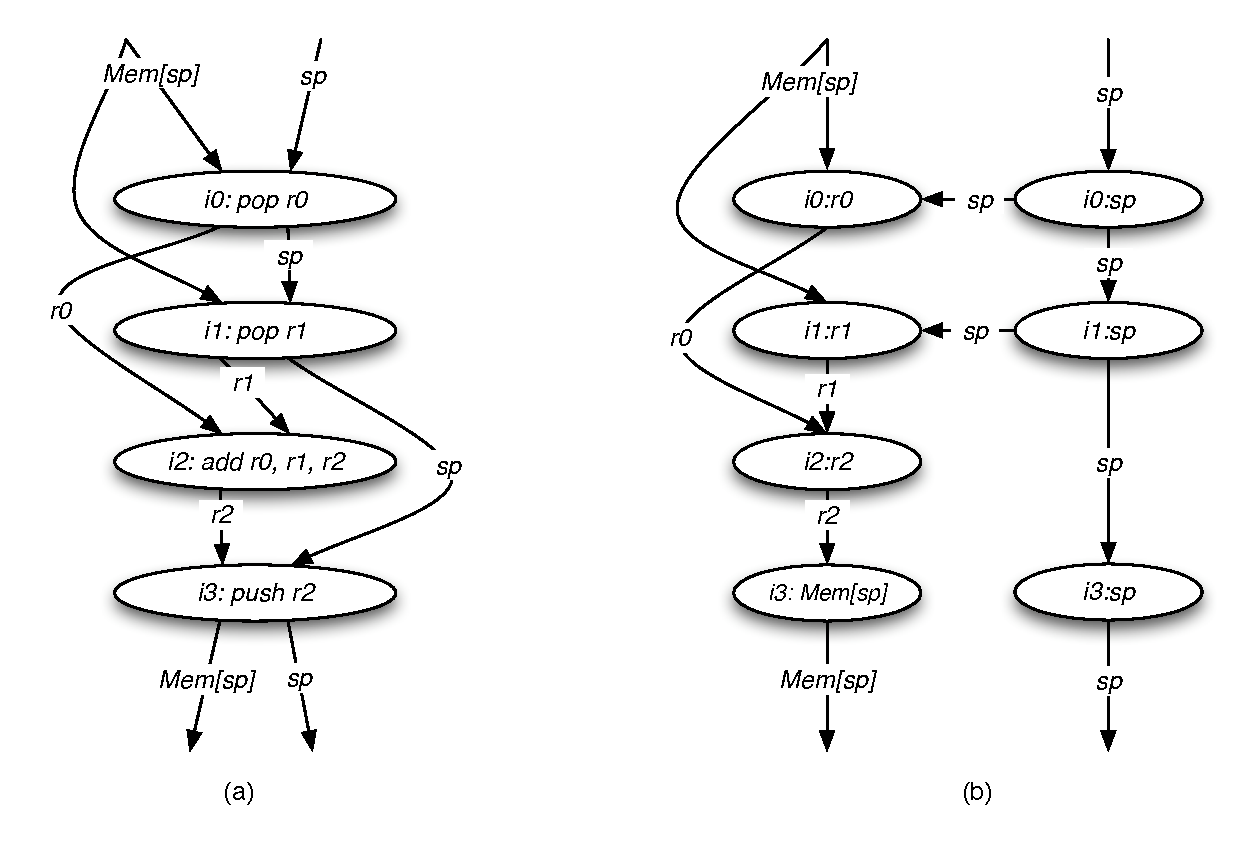
\epsfig{file=Operations_example,width=4in}
\caption{Example of DDG operations.  Two data dependence
graphs. Figure a) provides an example of the problems of representing
instructions as single nodes. In this graph it is possible for paths
to "cross" definitions; for example, there is a path from the
definition of r0 by i0 to the definition of sp (the stack pointer) by
i3, when in the actual program there is no such dependence. The DDG
shown in figure b) makes the intra-instruction data dependencies
explicit and thus removes the possibility of erroneous paths.}
\end{center}
\end{figure}

\section{Namespaces}

The classes described below are defined in the Dyninst:: and
Dyninst::DepGraphAPI:: namespaces. The Graph, Node, and Edge classes
are contained in the Dyninst:: namespace.  To access them a user
should refer to them using the Dyninst:: prefix (e.g.,
Dyninst::Graph). Alternatively, a user can add the C++ using keyword
above any reference to such objects (e.g., "using namespace
Dyninst;"). All other classes are defined under the
Dyninst::DepGraphAPI namespace and should be referred to
appropriately.

\section{API Reference}

This section describes the interface of the DepGraphAPI. Each of the
subsections represents a different interface.
        
\subsection{Shared Classes}

The Graph, Node, and Edge classes are written to be generic and
shareable between DyninstAPI components. We include the API for these
classes here.

\subsubsection{Graph}

\begin{description}

\item[void entryNodes(NodeIterator \&begin, NodeIterator \&end)] This method returns a range of nodes (defined by begin and end) such that 1) all nodes in the graph are reachable from the nodes in this range by traversing out-edges and 2) the range is minimal. The nodes included in this range may be virtual. 
\item[void exitNodes(NodeIterator \&begin, NodeIterator \&end)]
This method returns a range of nodes (defined by begin and end) such that 1) all nodes in the graph are reachable from the nodes in this range by traversing in-edges and 2) the range is minimal. The nodes included in this range may be virtual.
\item[void allNodes (NodeIterator \&begin, NodeIterator \&end)]
This method returns the range of all nodes in the graph.
\item[void printDOT(std::string fileName)]
This method generates a representation of the graph in DOT format.
\item[bool find(Address addr, NodeIterator \&begin, NodeIterator \&end)]
This method sets \texttt{begin} and \texttt{end} to point to a range
representing the nodes with a particular address. It returns true if
the range is non-empty. 
\item[void removeAnnotation()]
This method removes the graph from internal storage. Once all user handles to the graph are discarded the graph will be destroyed.
\end{description}

\subsubsection{Node}

\begin{description}
\item[bool hasInEdges()] This method returns true if the node has at
  least one in edge. 
\item[void ins(EdgeIterator \&begin, EdgeIterator \&end)]
This method returns the range of in edges to the node (edges that have the node as a target). 
\item[void ins(NodeIterator \&begin, NodeIterator \&end)]
This method is similar to the previous, but automatically traverses the edges and returns a range of source nodes. 
\item[bool hasOutEdges()] This method returns true if the node has at
  least one out edge. 
\item[void outs(EdgeIterator \&begin, EdgeIterator \&end)]
This method returns the range of out edges from the node (edges that have the node as a source). 
\item[void outs(NodeIterator \&begin, NodeIterator \&end)]
This method is similar to the previous, but automatically traverses the edges and returns a range of target nodes.
\item[void forwardClosure(NodeIterator \&begin, NodeIterator \&end)]
This method returns all nodes reachable from this node in the forward direction (by traversing out-edges).
\item[void backwardsClosure(NodeIterator \&begin, NodeIterator \&end)]
This method returns all nodes reachable from this node by traversing in-edges.
\item[std::string format()]
This method returns a textual representation of the node.
\item[bool isVirtual() ]
This method returns true if a node is virtual.
\end{description}

\subsubsection{PhysicalNode : Node}
\begin{description}
\item[Address addr()] This method returns the starting
offset of the code object (basic block, instruction, or operation) the
node represents.
\item[bool isVirtual()] This method returns false for physical nodes.
\end{description}

\subsubsection{VirtualNode : Node}
\begin{description}
\item[bool isVirtual()]
This method always returns true for virtual nodes.
\end{description}

\subsubsection{Edge}
\begin{description}
\item[Node::Ptr source()]
This method returns the source node of an edge.
\item[Node::Ptr target() ]
This method returns the target node of an edge.
\end{description}

\subsection{Data Dependence Graph}
\subsubsection{DDG}
\begin{description}
\item[DDG::Ptr analyze(BPatch\_function *func)]
This method creates and returns a DDG for the provided function.
\item[void formalParameterNodes(NodeIterator \&begin, NodeIterator \&end) ]
This method returns the range of all formal parameters to the function.
\item[void formalReturnNodes(NodeIterator \&begin, NodeIterator \&end)]
This method returns the range of all formal returns from the function.
\item[void actualParameterNodes(Address callAddr, NodeIterator \&begin, NodeIterator \&end) ]
This method returns the range of all actual parameters for the call instruction
at the given address.
\item[void actualReturnNodes(Address callAddr, NodeIterator \&begin, NodeIterator \&end)]
This method returns the range of all actual returns for the call instruction at
the given address.
\item[bool find(Address addr, Absloc::Ptr absloc, NodeIterator \&begin, NodeIterator \&end) ]
This method returns the range of nodes that fit the specific address
and absloc requirements. This range will contain at most one
element. It returns true if the range is non-empty, and false
otherwise. 
\end{description}

\subsubsection{Absloc}
\begin{description}
\item[std:string format()]
This method returns a textual representation of the abstract location. This representation is guaranteed to be unique for unique abstract locations.
\item[void getAliases(AbslocIterator \&begin, AbslocIterator \&end)]
If more than one Absloc may refer to the same abstract location (e.g., a particular stack slot and the representation of the entire stack) return any such aliases.
\item[bool isPrecise()]
This method returns true if the absloc does not contain any others; that is, if any aliases are more general than this one.
\end{description}

\subsubsection{OperationNode : PhysicalNode}
\begin{description}
\item[Absloc::Ptr absloc()]
This method returns the abstract location represented by this node.
\end{description}

\subsubsection{FormalParameterNode : VirtualNode}
\begin{description}
\item[Absloc::Ptr absloc()]
This method returns the abstract location represented by this node. 
\end{description}

\subsubsection{FormalReturnNode : VirtualNode}
\begin{description}
\item[Absloc::Ptr absloc()]
This method returns the abstract location represented by this node.
\end{description}

\subsubsection{ActualParameterNode : VirtualNode}
\begin{description}
\item[Absloc::Ptr absloc()]
This method returns the abstract location represented by this node.
\item[BPatch\_function *callee() ]
This method returns the callee function whose argument is represented by this node.
\end{description}

\subsubsection{ActualReturnNode : VirtualNode}
\begin{description}
\item[Absloc::Ptr absloc()]
This method returns the abstract location represented by this node.
\item[BPatch\_function *callee() ]
This method returns the callee function whose return is represented by this node.
\end{description}

\subsection{Control Dependence Graph}
\subsubsection{CDG}
\begin{description}
\item[CDG::Ptr analyze(BPatch\_function *func)]
This method creates and returns a CDG for the provided function.
<<<<<<< HEAD:depGraphAPI/doc/depGraphAPI.tex
\item[bool find(BPatch\_basicBlock *block, NodeIterator \&begin, NodeIterator \&end)]
This method returns the range of nodes representing the provided
block. This range will have at most one element. It returns true if
the range is non-empty and false otherwise. 
\item[bool find(Address addr, NodeIterator \&begin, NodeIterator
\&end)] This method returns the range of nodes containing the provided
address. It returns true if the range is non-empty and false
otherwise.
\end{description}

\subsubsection{BlockNode : PhysicalNode}
\begin{description}
\item[BPatch\_basicBlock *block() ]
This method returns the basic block represented by this node. 
\end{description}

\subsection{Program Dependence Graph}
\subsubsection{PDG}
\begin{description}
\item[PDG::Ptr analyze(BPatch\_function *func)]
Creates and returns a PDG for the provided function.
\item[find(Address addr, Absloc::Ptr absloc, NodeIterator \&begin, NodeIterator \&end) ]
This method returns the set of nodes that fit the specific address and absloc requirements. This node will be singular.
\end{description}

\subsection{Extended Program Dependence Graph}
\subsubsection{xPDG}
\begin{description}
\item[xPDG::Ptr analyze(BPatch\_function *func)]
Creates and returns an xPDG for the provided function.
\item[find(Address addr, Absloc::Ptr absloc, NodeIterator \&begin, NodeIterator \&end) ]
This method returns the set of nodes that fit the specific address and absloc requirements. This node will be singular.
\end{description}

\section{Implementation Status}

This release of the DepGraphAPI is a public beta and has limited
platform support and implementation features. These limitations are as
follows:
\begin{itemize}
\item Platforms: the DepGraphAPI is implemented for IA-32 and
  x86-64. This is primarily due to a dependence on the InstructionAPI.
\item Limited operator node support. We currently do not identify
  intra-instruction dependences between used and defined abstract
  locations. Instead, there is a complete interconnection between
  these. 
\end{itemize}


\section{Building DepGraphAPI}
This appendix describes how to build DepGraphAPI from source code,
which can be downloaded from http://www.paradyn.org or
http://www.dyninst.org.

\subsection{Building on Unix}
The beta of the DepGraphAPI depends on the DyninstAPI. It is currently
packaged with the DyninstAPI source tree. It can be built using the
DepGraphAPI make target once the DyninstAPI has been built and
installed.

\end{document}
